\documentclass[12pt,a4paper]{article}

\usepackage[width=200mm,height=290mm,centering]{geometry}

\usepackage{mathptmx}
\usepackage{palatino}

\usepackage{graphicx}
\usepackage{xcolor}
\usepackage{tikz}
\usepackage[hidelinks]{hyperref}

\pagestyle{empty}

\newcommand{\logo}{\makebox[56mm][c]{\rule{0mm}{66mm}\raisebox{12mm}{
\includegraphics[width=48mm]{images/logo.png}}}}

\pagecolor{yellow!5}

\begin{document}
\sffamily

\vspace*{-20mm}\hspace*{-15mm}
\begin{tikzpicture}(20,7)
\shade[left color=black!25!red, right color=black!25!blue] (-8,0) rectangle (18,7);
\node at (-4,3){\logo};
\node at (10,3){\logo};
\end{tikzpicture}

% \begin{minipage}{1.0\linewidth}
% \colorbox{blue!50}{
\includegraphics[width=50mm]{images/logo.png}}
% \end{minipage}

\vfill

\begin{center}
\href{https://alevisdanse.github.io}{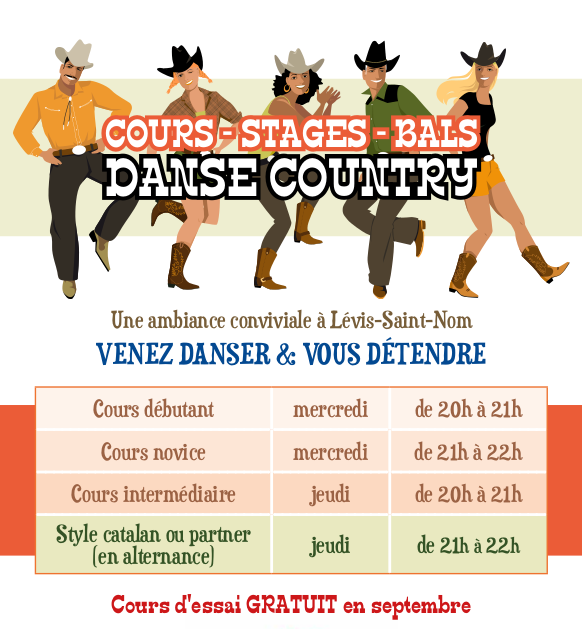
\includegraphics{images/flyerLCLD.png}}

\vfill\vfill

\href{https://alevisdanse.github.io}{\raisebox{-20mm}{\includegraphics[width=40mm]{images/qr-code.png}}}
\qquad
\begin{minipage}[c]{0.37\textwidth}
\Huge\color{black!50!blue}  \href{https://alevisdanse.github.io}{Plus d'information sur notre page web $\longleftarrow$}
\end{minipage}

\end{center}

\end{document}
